\section{Emil Wajda}

Table ~\ref{tab:losowe liczby} to:
\begin{table}[htbp]
\centering
\begin{tabular}{|c|c|c|c|c|}
\hline
\textbf{4234}  & \textbf{223}   & \textbf{44.4} & \textbf{4231} & \textbf{5323} \\ \hline
\textbf{12356} & \textbf{6723}  & \textbf{4636} & \textbf{6346} & \textbf{2134} \\ \hline
\textbf{2361}  & \textbf{62346} & \textbf{6246} & \textbf{646}  & \textbf{423}  \\ \hline
\textbf{6723}  & \textbf{2515}  & \textbf{523}  & \textbf{234}  & \textbf{6234} \\ \hline
\end{tabular}
\caption{Losowe liczby}
\label{tab:losowe liczby}
\end{table}

\vspace{2 cm}

To jest zdjęcie słodkiego psa (zobacz Figure~\ref{fig:labrador}).
\begin{figure}[htbp]
    \centering
    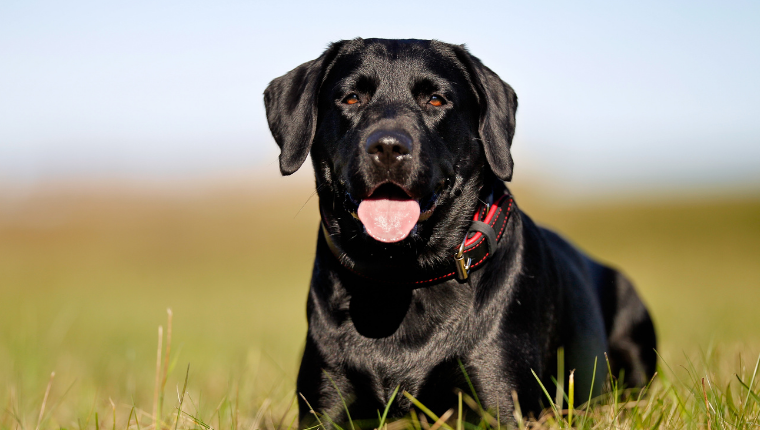
\includegraphics[width=0.8\textwidth]{pictures/labrador.png}
    \caption{czarny pies}
    \label{fig:labrador}
\end{figure}

Wzór na pole koła o promieniu r: $$P= \pi r^2$$

Przykład listy numerowanej:
\begin{enumerate}
    \item item I
    \item item II
    \item item III
\end{enumerate}

Przykład listy nienumerowanej:
\begin{itemize}
    \item item I
    \item item II
    \item item III
\end{itemize}

\begin{center}
Labradory to rasa \textbf{dużych} psów o \textbf{przyjacielskim} wyglądzie. Sylwetkę tego czworonoga można łatwo rozpoznać: \textit{przylegające uszy, szeroka klatka piersiowa, mocna szyja, zwarte łapy i gruby u nasady ogon, który zwęża się ku końcowi}. \underline{Samce labradorów są większe od samic.}
\end{center}

\begin{flushleft}
    Labrador retriever ma \textbf{mocną i zwartą budowę ciała}, szeroką czaszkę, dobrze rozwiniętą klatkę piersiową, \underline{mocne i szerokie kończyny tylne}. \textit{Jego sierść jest gęsta, nieco szorstka w dotyku, krótka i przylegająca. Na uwagę zasługuje bardzo gęsty podszerstek, który nie przepuszcza wilgoci}. Sierść jest jednobarwna.
\end{flushleft}

Zdjęcie nr: \ref{fig:labrador} ukazuje czarnego labradora.\par
Tabela nr: \ref{tab:losowe liczby} przedstawia losowe liczby.
